\documentclass[12pt,a4paper,UTF8]{ctexart}




%设置页边距
\usepackage{geometry}
\geometry{left=2.5cm,right=2.5cm,top=2.5cm,bottom=2.5cm}




%需要用到的扩展包
\usepackage{xeCJK,amsmath,paralist,enumerate,booktabs,multirow,graphicx,float,subfig,setspace,listings,lastpage,hyperref}
\usepackage{fancyhdr}




%设置页眉页脚以及页码
\pagestyle{fancy}
\rhead{示波器的使用}
\lhead{大学基础物理实验报告}
\cfoot{Page\thepage/\pageref{LastPage}}
\rfoot{\today}




%报告中用到的图片存放在这个tex文件所在目录中的figures子目录中
\graphicspath{{figures/}}









%报告开始
\begin{document}
	
	
	
	
	%设置课程标题
	\begin{center}
		\heiti\LARGE{《大学基础物理实验》课程实验报告}
	\end{center}
	
	
	
	
	%设置实验人信息以及实验时间表格
	
	
	\begin{center}
		\begin{tabular}{lcr}
			
			{\songti 姓名及学号:蒋丰毅2211082}  \quad 专业:工科试验班 \quad 年级:22级 \quad 座号:10\\
			{\songti  学院:软件学院 \quad 实验组别:C组\quad 实验时间:2023年3月24日~星期五~上午}\\
			
			
		\end{tabular}
	\end{center}
	\vspace{-0.2cm}
	{\noindent}	 \rule[-10pt]{17.5cm}{0.05em}\\
	
	\vspace{-0.4cm}
	
	
	
	
	
	
	%实验题目
	\begin{center}
		\LARGE\textbf{示波器的使用}
	\end{center}
	
	
	
	%实验原理
	\subsection*{[仪器与用具]}
	\par 1.1仪器品牌与型号:
	\par 示波器:普源DS1102E,信号发生器:F05函数发生器
	\par 1.2电阻阻值:1k$\Omega$,电容值:0.1$\mu F$
	
	\subsection{[基本使用]}
	\par 将信号源($1KHz,3Vp-p$)和变压器电压同时输出到示波器,分别稳定并显示适当的波形。重点熟悉触发对波形的作用。
	
	\subsection{[实验数据]}
	\subsubsection*{信号源和变压器测量}
	\begin{table}[!htbp]
		\centering
		\caption{实验测量数据}
	\begin{tabular}{|p{2cm}|p{2cm}|p{2cm}|p{2cm}|}
		\hline
		\rule{0pt}{16pt} 信号源 & 自动测量 & 光标测量 & 读格测量 \\ \hline
		\rule{0pt}{16pt} 电压  & 6.08V & 6.00V&6.00V\\ \hline
		\rule{0pt}{16pt} 周期  & 20ms  & 20ms & 20ms\\ \hline
		\rule{0pt}{16pt} 频率  & 50Hz  & 50Hz &50Hz \\ \hline
		\rule{0pt}{16pt} &      &      &      \\ \hline
		\rule{0pt}{16pt} 变压器 & 自动测量 & 光标测量 & 读格测量 \\ \hline
		\rule{0pt}{16pt} 电压  & 6.24V& 6.24V     &6.24V\\ \hline
		\rule{0pt}{16pt} 周期  & 1.00ms  & 1.00ms&1.00ms\\ \hline
		\rule{0pt}{16pt} 频率  &  1000Hz& 1000Hz&1000Hz\\ \hline
	\end{tabular}
\end{table}
\par 实验图片如下:
\clearpage
		\begin{figure}[htbp]
		\centering
		\begin{minipage}[t]{0.49\textwidth}
			\centering
			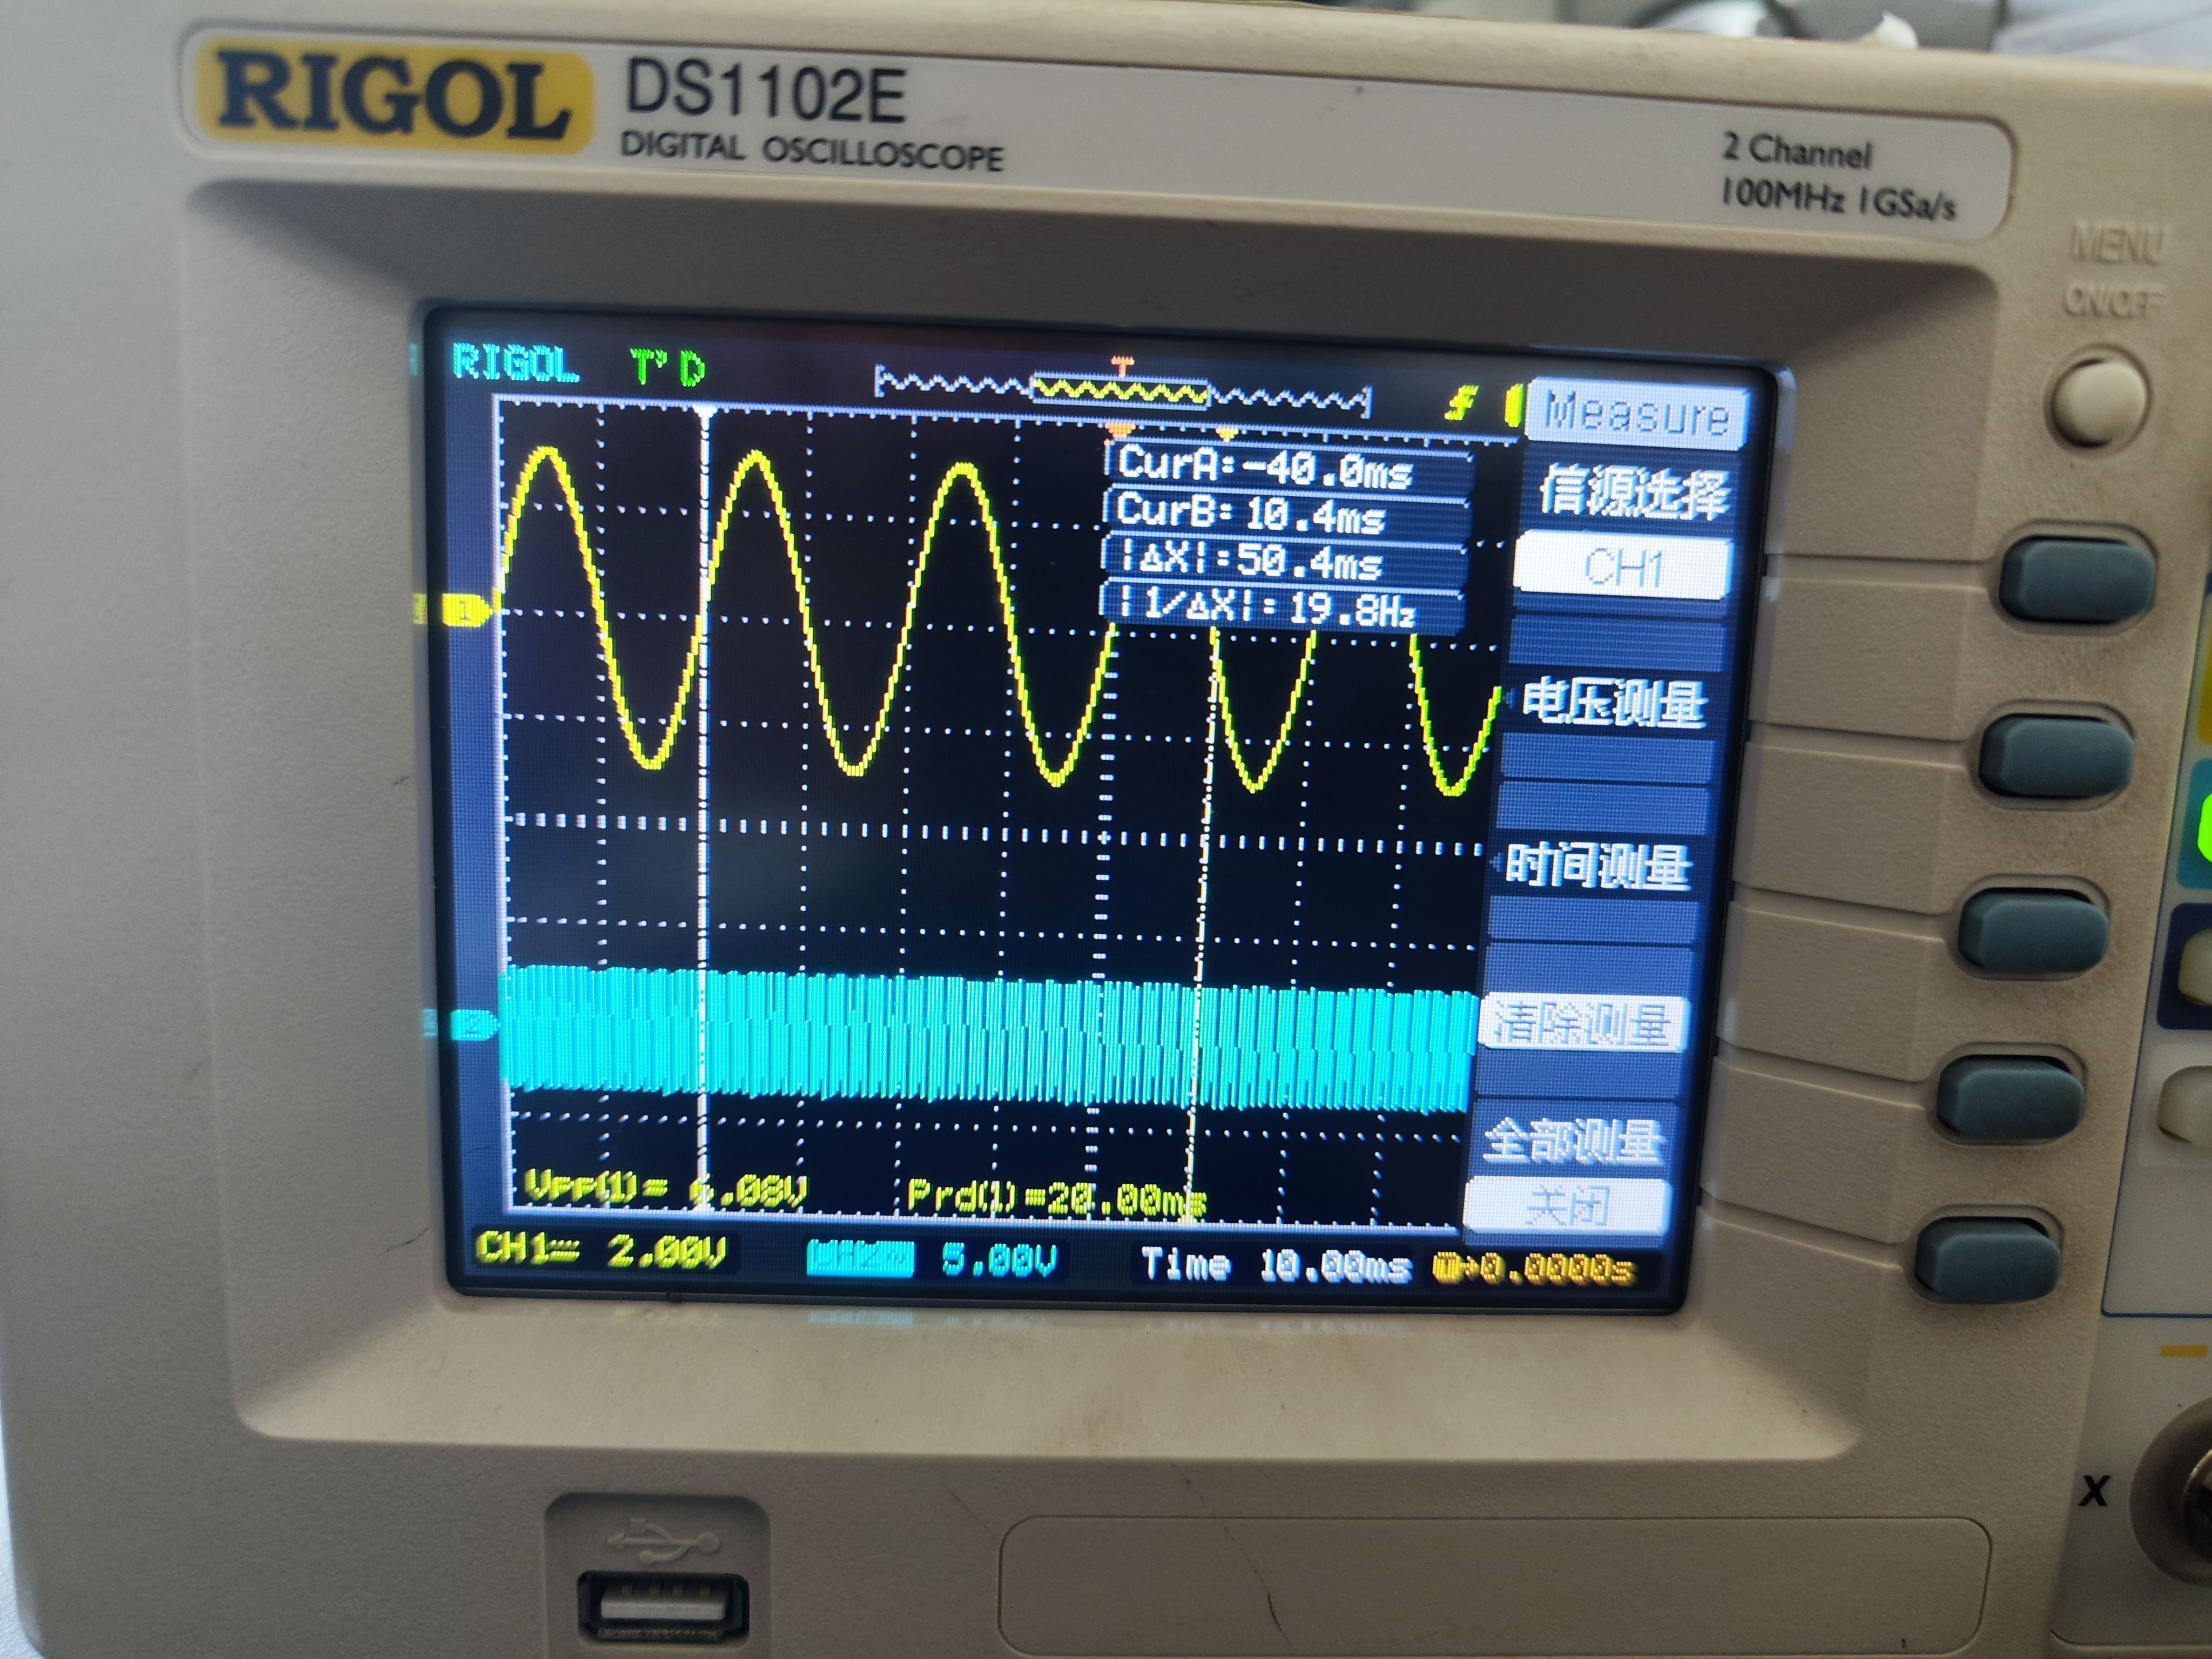
\includegraphics[width=5cm]{图片1}
			\caption{变压器}
		\end{minipage}
		\begin{minipage}[t]{0.49\textwidth}
			\centering
			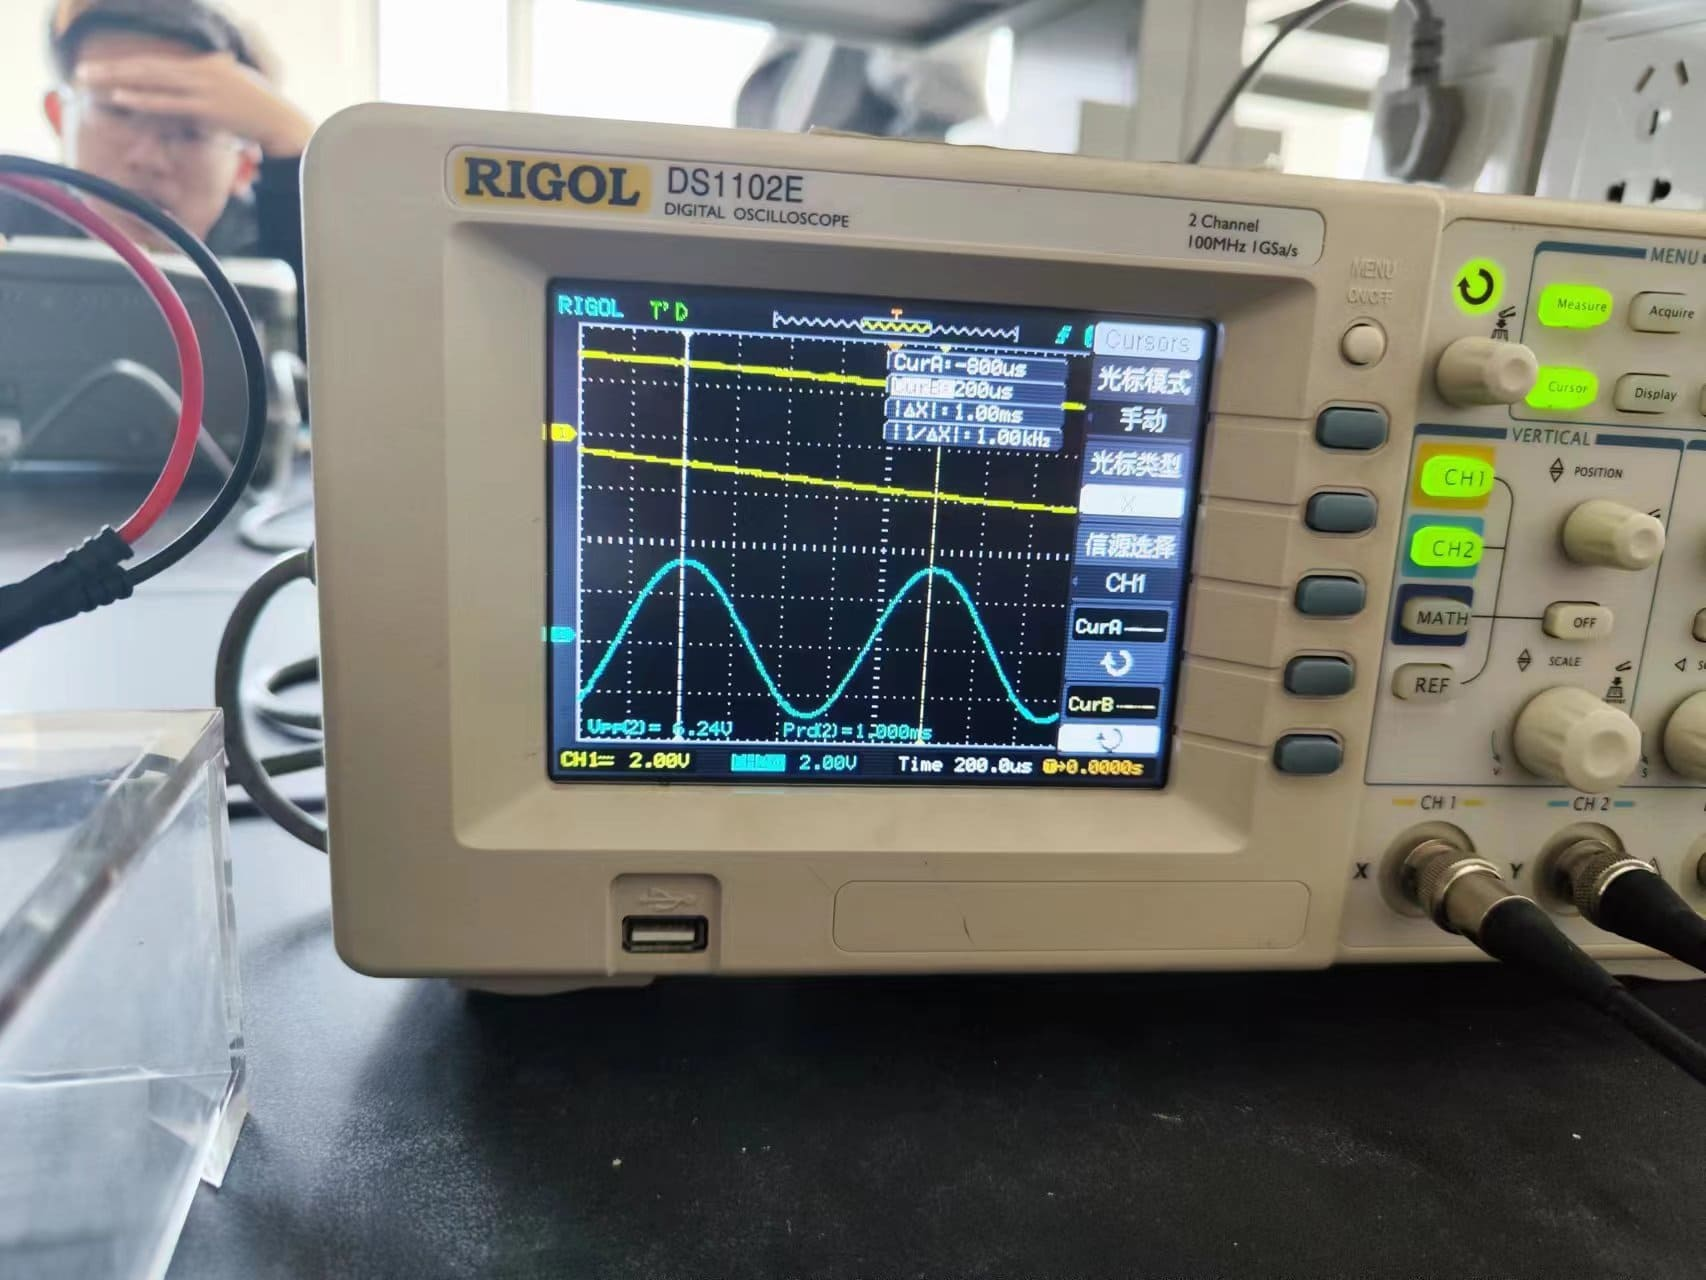
\includegraphics[width=5cm]{图片2}
			\caption{信号源}
		\end{minipage}
	\end{figure}
	\subsubsection*{李萨如图形测量法}
	\begin{table}[!htbp]
		\centering 
		\begin{tabular}{|c|c|c|c|c|}
			\hline
			\rule{0pt}{20pt}$\frac{\mbox{与水平线的交点数}}{\mbox{与竖直线交点数}}=\frac{n_2}{n_1}$    & 1 & 2 & 3 & 4  \\ \hline
			\rule{0pt}{20pt}函数发生器频率 & 49.97 & 99.93 & 149.90 & 200.08   \\ \hline
			\rule{0pt}{20pt}算出的市电频率 &  49.97& 49.97 & 49.97 &50.02 \\ \hline
		\end{tabular}
	\end{table}
	\par 计算得到平均市电频率为49.98Hz
	\subsection*{[测量RC电路的相位差]}
	\par 连接电路,将信号发生器频率设定为$f=1.59KHz$
	\subsubsection*{椭圆法}
	$$
	|\theta|=\arcsin\frac{2x_0}{2x_m}=\arcsin\frac{2.80}{4.00}\approx0.775
	$$
	\subsubsection*{位移法}
	\[
	\theta = \frac{l}{l_0}\times 360^o = \frac{224}{312}\approx0.718
	\]

	\subsubsection*{[思考题]}
	\par 嘻嘻,没有思考题
	
	
	
	
	
	
\end{document}
